\section{信号的基本概念与数学基础}

这一章主要涉及信号的基本概念与数学基础。

\subsection{信号的概念}

\begin{definition}[信号]
    \bd{信号}是人对物理世界的一种\bd{观察}。
    \bd{观察}是人通过\bd{传感器}对物理世界的一种\bd{测量}。
    \bd{传感器}是把一种物理变化转换成另一种物理变化的装置。
    \bd{测量}是指用一种物理量来表示另一种物理量。

    信号是反映(或载有)信息的物理量,是系统直接进行加工、变换以实现通信的对象。
    信号是信息的表现形式,信息则是信号里所蕴含的内容
\end{definition}

\begin{example}[传感器]
    传感器的种类繁多。例如:
    \begin{enumerate}
        \item 光
            \begin{itemize}
                \item 数码相机:光能产生电信号。
            \end{itemize}
        \item 空气振动
            \begin{itemize}
                \item 麦克风:空气的振动能产生电信号。
            \end{itemize}
        \item 温度
            \begin{itemize}
                \item 热敏电阻:阻值随温度变化。
                \item 热电偶:由对温度反应不同的两种金属制成,温差导致电压。
            \end{itemize}
    \end{enumerate}

    除此之外,还有加速度传感器、压力传感器、流量传感器等。
    值得注意的是,耳朵(图 \ref{fig:ear})就是一种传感器。
    \begin{figure}[H]
        \centering
        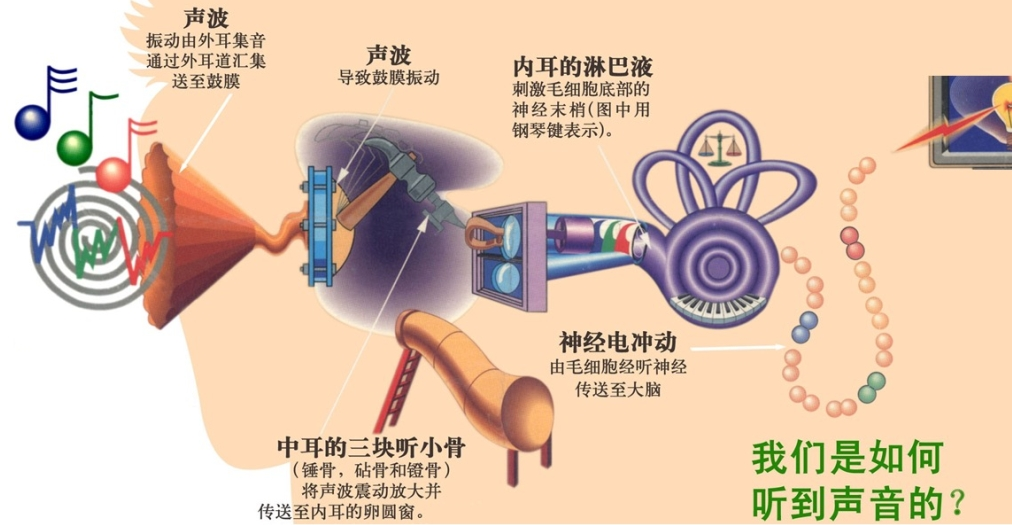
\includegraphics[width=0.5\textwidth]{chap1/img/ear.png}
        \caption{耳朵是一种传感器}
        \label{fig:ear}
    \end{figure}
\end{example}

\begin{definition}[信号处理]
    \bd{信号处理}是对信号进行变换、分析和综合等处理过程的统称。
    信号处理的目的是
    \begin{itemize}
        \item 去伪存真:去除信号中冗余的和次要的成分。
        \item 特征抽取:把信号变成易于进行分析和识别的形式。
        \item 编码解码:把信号变成易于传输、交换与存储的形式(编码),
            或从编码信号中恢复出原始信号(解码)。
    \end{itemize}
\end{definition}

\begin{example}[数字信号处理(DSP)系统]
    由于数字系统的工作具有\bd{可预测性}和\bd{可重复性},
    而模拟系统是由元器件搭建而成的电路,制造误差范围大,
    特性随温度(温度漂移)和时间变化(老化)。
    因此,\bd{数字信号处理(DSP)系统}应运而生。

    DSP 系统的特点有:
    \begin{itemize}
        \item 体积小,功耗低:数字系统通常由集成电路构成,这些电路可以在非常小的尺寸上集成大量的电子元件。这不仅减少了设备的体积,也降低了功耗,这对于移动终端的发展尤为重要。
        \item 有高度的灵活性:数字系统可以通过软件编程来实现多种功能,这使得它们非常灵活。修改程序中的一些语句就能修改系统的行为,而无需改变硬件。
        \item 模拟信号与数字信号的不同:
            \begin{itemize}
                \item 模拟音频以模拟电压的幅度表示声音强弱。
                \item 数字音频是有限数值表示的离散数字序列。
            \end{itemize}
    \end{itemize}
    例如,修改``抽样频率'',就可以改变数字音频音高/音速。
\end{example}

\subsection{信号的描述}

信号的描述有两种方式:数学描述和波形描述。

\begin{definition}[数学描述]
    信号的\bd{数学描述}是指,使用具体的数学表达式,
    把信号描述为一个或若干个自变量的函数或序列的形式。
\end{definition}

\begin{definition}[波形描述]
    信号的\bd{波形描述}是指,按照函数随自变量的变化关系,把信号的波形画出来。
\end{definition}

\begin{note}
    在画波形描述时,需要写清\bd{横纵坐标标识},并\bd{标出原点}。
\end{note}

\begin{example}
    以下是信号的数学描述和波形描述的例子:
    \begin{itemize}
        \item 数学描述:$f(t) = \sin t, x(n) = a^nu(n)$。
        \item 波形描述:$\sa(t) = \frac{\sin t}{t}$ 的示意图如图 \ref{fig:sa-t-wave-description}。
    \end{itemize}
    \begin{figure}[H]
        \centering
        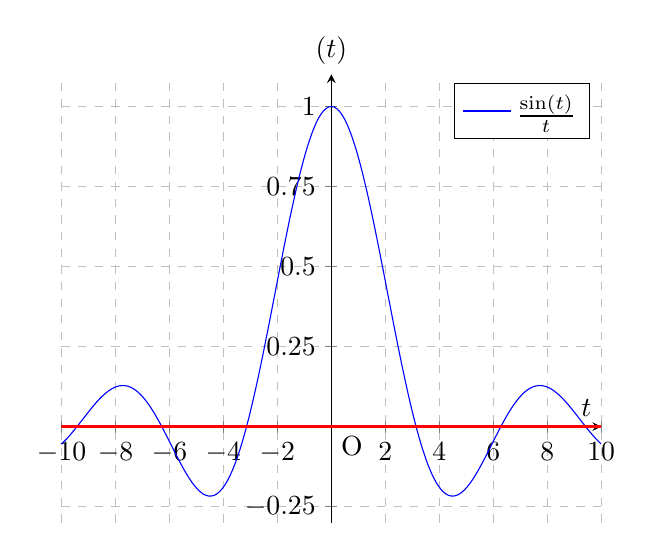
\begin{tikzpicture}
            \begin{axis}[
                axis lines = middle,
                xlabel = {$t$},
                ylabel = {$\sa(t)$},
                ylabel style={at={(rel axis cs:0.5, 1)}, anchor=south},
                xmin = -10, xmax = 10,
                ymin = -0.3, ymax = 1.1,
                xtick = {-10, -8, -6, -4, -2, 0, 2, 4, 6, 8, 10},
                ytick distance = 0.25,
                grid = major,
                grid style = dashed,
            ]
            \addplot[domain=-10:10, samples=100, smooth, blue] {sin(deg(x))/x};
            \addlegendentry{$\frac{\sin(t)}{t}$}
            \addplot[domain=-10:10, red, thick] {0};
            \node at (axis cs:0, 0) [anchor=north west] {O};
            \end{axis}
        \end{tikzpicture}
        \caption{$\sa(t) = \frac{\sin t}{t}$ 的波形描述}
        \label{fig:sa-t-wave-description}
    \end{figure}
\end{example}

\begin{example}[时域波形与频谱图]
    时域波形与频谱图如图 \ref{fig:wave-spectrum} 所示。
    \begin{figure}[H]
        \centering
        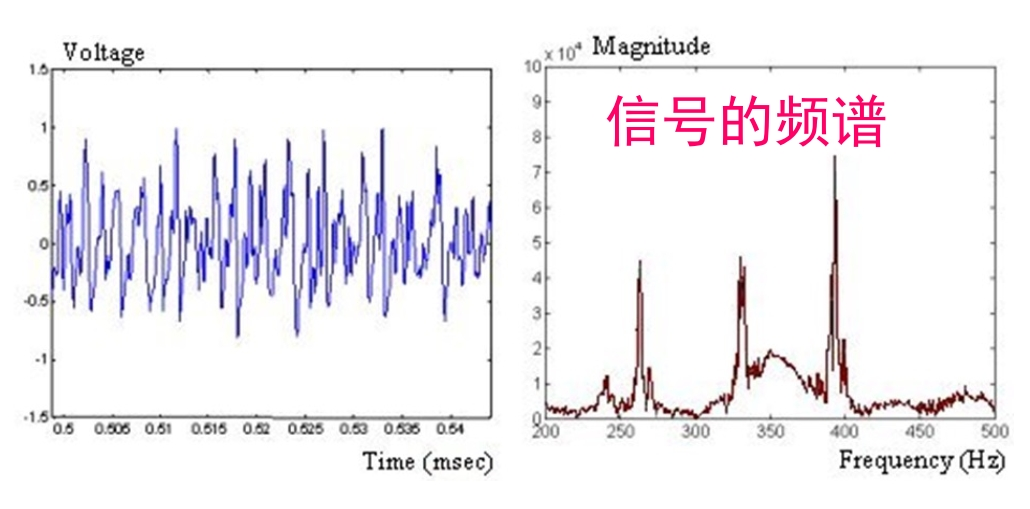
\includegraphics[width=0.5\textwidth]{chap1/img/wave-spectrum.png}
        \caption{左侧为时域波形,右侧为频谱图}
        \label{fig:wave-spectrum}
    \end{figure}
\end{example}

\begin{definition}[确定信号与随机信号]
    任意给定一个自变量的值,如果可以唯一确定其信号和取值,则该信号是\bd{确定信号}。
    否则,如果取值是不确定的随机值,则是\bd{随机信号}。
\end{definition}

\begin{definition}[周期信号]
    如果存在正数 $T$,使得对于任意 $t$ 都有 $f(t) = f(t + T)$,
    则称 $f(t)$ 为\bd{周期信号}。
    周期信号的\bd{周期} $T$ 是使得 $f(t) = f(t + T)$ 成立的最小正数。
\end{definition}

\begin{remark}
    非周期信号可以看做是周期为无穷大的周期信号。
\end{remark}

\begin{example}[正弦信号与余弦信号]
    正弦信号与余弦信号是最常见的周期信号。它们的数学描述如下:
    \begin{itemize}
        \item 正弦信号:$f(t) = K\sin(\omega t + \theta)$。
        \item 余弦信号:$f(t) = K\cos(\omega t + \theta)$。
    \end{itemize}
    其中 $K > 0$ 为振幅,$\omega$ 为角频率,$\theta$ 为初相位。
\end{example}

\begin{example}[$\sa$ 函数]
    $\sa$ 函数的数学描述如下:
    \begin{align*}
        \sa(t) = \frac{\sin t}{t}.
    \end{align*}
    它有以下性质:
    \begin{itemize}
        \item $\sa(t)$ 是偶函数。
        \item $\sa(t)$ 的零点为 $t = k\pi, k \ne 0$。
        \item 过零区间:除原点附近的过零区间宽度为 $2\pi$ 外,
            其他过零区间宽度均为 $\pi$。
        \item $\int_{-\infty}^{0}\sa(t)\D{t} = \int_{0}^{+\infty}\sa(t)\D{t} = \frac{\pi}{2}$,
            $\int_{-\infty}^{+\infty}\sa(t)\D{t} = \pi$。
    \end{itemize}
\end{example}

\begin{note}
    一定要注意,$\sa(t)$ 在 $t = 0$ 处的取值是 $1$,
    而不是 $0$。$\sa(t)$ 的零点不包括 $t = 0$。
\end{note}

\begin{example}[指数信号]
    指数信号是一种常见的非周期信号。它的数学描述如下:
    \begin{align*}
        f(t) = K\mathe^{\alpha t}.
    \end{align*}
    其中 $K > 0$ 为振幅,$\alpha$ 为参数。
    对于 $\alpha$ 的符号而言:
    \begin{itemize}
        \item 若 $\alpha > 0$,则信号随时间\bd{增强}。
        \item 若 $\alpha = 0$,则信号为\bd{直流信号}。
        \item 若 $\alpha < 0$,则信号随时间\bd{减弱}。
    \end{itemize}
    对于 $\alpha$ 的绝对值大小而言:
    \begin{itemize}
        \item 若 $\alpha$ 的绝对值大,则信号变化速度\bd{快}。
        \item 若 $\alpha$ 的绝对值小,则信号变化速度\bd{慢}。
    \end{itemize}
\end{example}

\begin{remark}
    指数信号微分或积分后仍然是指数信号。
\end{remark}

\subsection{信号的数学基础}

\subsubsection{欧拉公式}

\begin{definition}[实值信号与复值信号]
    如果信号的取值是实数,则称为\bd{实值信号},简称\bd{实信号}。
    如果信号的取值是复数,则称为\bd{复值信号},简称\bd{复信号}。
\end{definition}

\begin{theorem}[欧拉公式]
    对于任意的 $\theta \in \set{R}$,都有以下的恒等式成立:
    \begin{align*}
        \mathe^{\mathi \theta} = \cos \theta + \mathi \sin\theta.
    \end{align*}

    特别地,当 $\theta = \pi$ 时,有 $\mathe^{\mathi\pi} + 1 = 0$。
\end{theorem}

\begin{proof}
    \nl{(欧拉公式的泰勒级数法证明)} 分别将 $\mathe^x, \sin x, \cos x$ 进行泰勒展开,得:
    \begin{align*}
        \mathe^x &= \sum_{k = 0}^{+\infty}\frac{x^k}{k!}, \\
        \sin x   &= \sum_{k = 0}^{+\infty}\frac{(-1)^kx^{2k + 1}}{(2k + 1)!}, \\
        \cos x   &= \sum_{k = 0}^{+\infty}\frac{(-1)^kx^{2k}}{(2k)!}.
    \end{align*}
    考虑到 $\mathi^2 = -1$,因此可以将 $\cos x$ 和 $\mathi\sin x$ 写成以下形式:
    \begin{align*}
        \cos x &= \sum_{k = 0}^{+\infty}\frac{(\mathi^2)^kx^{2k}}{(2k)!}
                = \sum_{k = 0}^{+\infty}\frac{(\mathi x)^{2k}}{(2k)!}, \\
        \mathi\sin x &= \mathi\sum_{k = 0}^{+\infty}\frac{(\mathi^2)^kx^{2k + 1}}{(2k + 1)!}
                = \sum_{k = 0}^{+\infty}\frac{(\mathi x)^{2k + 1}}{(2k + 1)!}.
    \end{align*}
    故
    \begin{align*}
        \mathe^{\mathi x} & = \sum_{k = 0}^{+\infty}\frac{(\mathi x)^k}{k!} \\
        & = \sum_{k = 0}^{+\infty}\frac{(\mathi x)^{2k}}{(2k)!} + 
            \sum_{k = 0}^{+\infty}\frac{(\mathi x)^{2k + 1}}{(2k + 1)!} \\
        & = \cos x + \mathi \sin x.
    \end{align*}
\end{proof}

\begin{corollary}
    由欧拉公式可得,对于任意的 $\theta \in \set{R}$:
    \begin{align*}
        \sin \theta & = \frac{\mathe^{\mathi\theta} - \mathe^{-\mathi\theta}}{2\mathi}, \\
        \cos \theta & = \frac{\mathe^{\mathi\theta} + \mathe^{-\mathi\theta}}{2}.
    \end{align*}
\end{corollary}

\begin{example}[复值信号的图示]
    如果将 $\mathe^{\mathi \varphi}$ 看成一个复平面上的向量,
    则它的模长为 $1$,辐角主值为 $\varphi$,
    如图 \ref{fig:euler-formula-imaginary-plane} 所示。
    \begin{figure}[H]
        \centering
        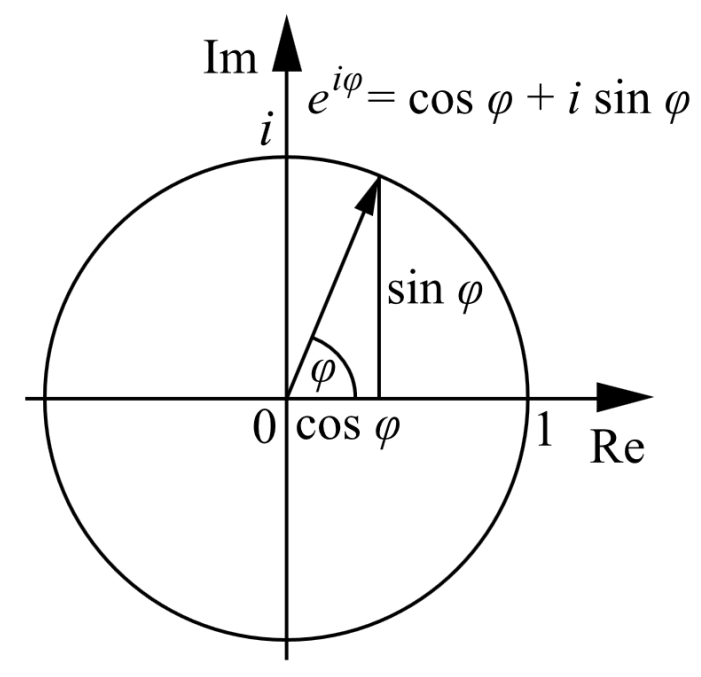
\includegraphics[width=0.5\textwidth]{chap1/img/euler-formula-imaginary-plane.png}
        \caption{$\mathe^{\mathi \varphi}$ 在复平面上的表示}
        \label{fig:euler-formula-imaginary-plane}
    \end{figure}

    如果使 $\varphi$ 随着时间 $t$ 的变化而变化,则画出三维图像(纵轴为时间)
    如图 \ref{fig:euler-formula-imaginary-signals.png} 所示。
    \begin{figure}[H]
        \centering
        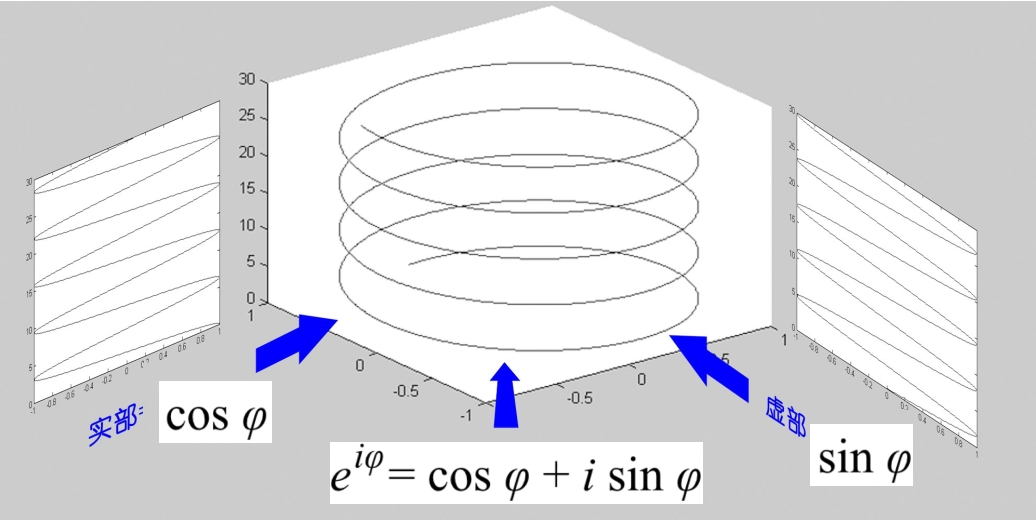
\includegraphics[width=0.5\textwidth]{chap1/img/euler-formula-imaginary-signals.png}
        \caption{$\mathe^{\mathi \varphi}$ 随时间的变化的在三维空间中的轨迹}
        \label{fig:euler-formula-imaginary-signals.png}
    \end{figure}
\end{example}

\begin{example}[复值信号在电磁场中的应用]
    由于电场和磁场互相垂直,所以可以用复值信号的实数部分和虚数部分分别表示电场与磁场信号。
\end{example}

\begin{proof}
    \nl{(欧拉公式的微分法证明)} 设有函数
    \begin{align*}
        f(x) = \frac{\cos x + \mathi \sin x}{\mathe^{\mathi x}}.
    \end{align*}
    则
    \begin{align*}
        \frac{\D{f}}{\D{x}} & = \frac{(-\sin x + \mathi \cos x)\mathe^{\mathi x}
                    - (\cos x + \mathi \sin x)\mathi \mathe^{\mathi x}}
                    {\mathe^{2\mathi x}} \\
        & = \frac{\mathe^{\mathi x}(-\sin x + \mathi \cos x - \mathi \cos x + \sin x)}{\mathe^{2\mathi x}} \\
        & = 0.
    \end{align*}
    因此 $f(x)$ 为常函数,故 $f(x) = f(0) = 1$。
    此即 $\mathe^{\mathi x} = \cos x + \mathi \sin x$。
\end{proof}

\begin{definition}[复指数信号]
    形如 $f(t) = K\mathe^{st}$,其中 $K \in \set{R}, s \in \set{C}$ 为参数,$t \in \set{R}$ 为自变量,
    这样的信号被称为\bd{复指数信号}。
\end{definition}

\begin{property}[复指数信号与正余弦信号之间的关系]
    不妨设 $s = \sigma + \mathi\omega$,其中 $\sigma, \omega \in \set{R}$。则复指数信号
    \begin{align*}
        f(t) & = K\mathe^{st} \\
        & = K\mathe^{(\sigma + \mathi\omega)t} \\
        & = K\mathe^{\sigma t} \cdot \mathe^{\mathi \omega t} \\
        & = K\mathe^{\sigma t} \cdot (\cos \omega t + \mathi \sin \omega t).
    \end{align*}

    固定 $K, \sigma, \omega$ 中的两个,做出第三个关于 $t$ 的变化图像如下:
    \begin{itemize}
        \item 固定 $\sigma = 0.2, \omega = 1$,$K$ 变化:图 \ref{fig:complex-exponential-signal-k-vary}。
        \item 固定 $K = 1, \omega = 1$,$\sigma$ 变化:图 \ref{fig:complex-exponential-signal-sigma-vary}。
        \item 固定 $K = 1, \sigma = 0.2$,$\omega$ 变化:图 \ref{fig:complex-exponential-signal-omega-vary}。
    \end{itemize}
    \begin{figure}[H]
        \centering
        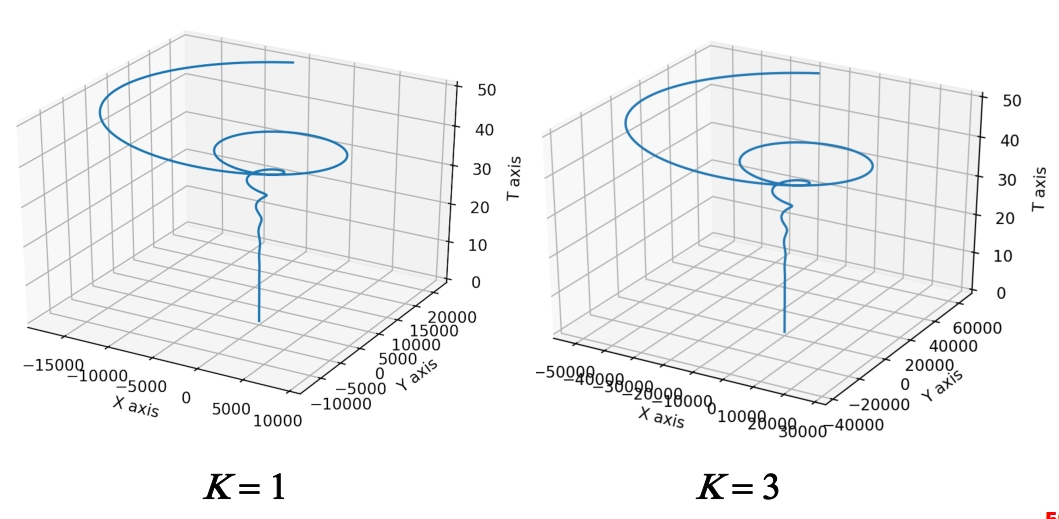
\includegraphics[width=0.5\textwidth]{chap1/img/complex-exponential-signal-k-vary.png}
        \caption{固定 $\sigma = 0.2, \omega = 1$,$K$ 变化}
        \label{fig:complex-exponential-signal-k-vary}
    \end{figure}
    \begin{figure}[H]
        \centering
        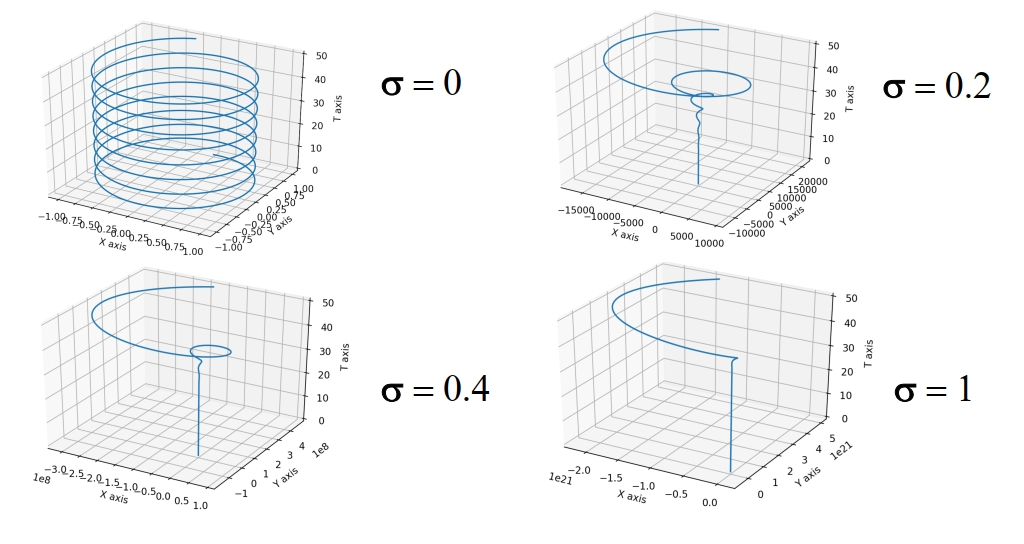
\includegraphics[width=0.5\textwidth]{chap1/img/complex-exponential-signal-sigma-vary.png}
        \caption{固定 $K = 1, \omega = 1$,$\sigma$ 变化}
        \label{fig:complex-exponential-signal-sigma-vary}
    \end{figure}
    \begin{figure}[H]
        \centering
        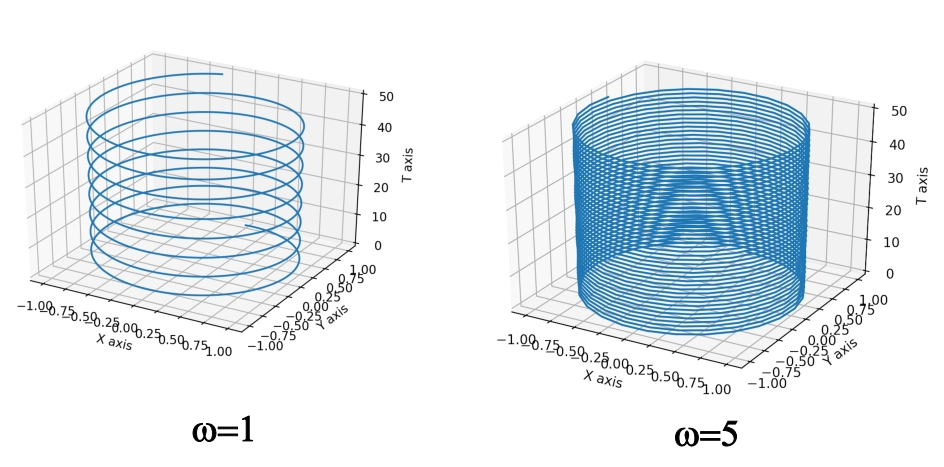
\includegraphics[width=0.5\textwidth]{chap1/img/complex-exponential-signal-omega-vary.png}
        \caption{固定 $K = 1, \sigma = 0.2$,$\omega$ 变化}
        \label{fig:complex-exponential-signal-omega-vary}
    \end{figure}
\end{property}

\subsubsection{函数分解}

\begin{definition}[正交基]
    设 $V$ 为欧式空间,非零向量 $\alpha_1, \alpha_2, \cdots, \alpha_m \in V$。
    \begin{enumerate}
        \item 如果它们两两正交,则称之为\bd{正交向量组}。
            一个较为显然的事实是,$n$ 维欧式空间中正交向量组所含向量个数 $\le n$。
        \item $n$ 维欧式空间中,由 $n$ 个向量构成的正交向量组称为\bd{正交基}。
        \item 由单位向量构成的正交基称为\bd{标准正交基}。
    \end{enumerate}
\end{definition}

\begin{example}
    在标准欧式空间 $\set{R}^3$ 中,向量组
    \begin{align*}
        \beta_1 = (0, 1, 0),
        \quad \beta_2 = (\frac{\sqrt{2}}{2}, 0, \frac{\sqrt{2}}{2}),
        \quad \beta_3 = (\frac{\sqrt{2}}{2}, 0, -\frac{\sqrt{2}}{2})
    \end{align*}
    是一个标准正交基。这是因为
    \begin{align*}
        \beta_1 \cdot \beta_2 = \beta_1 \cdot \beta_3 = \beta_2 \cdot \beta_3 = 0,
    \end{align*}
    且
    \begin{align*}
        \|\beta_1\| = \|\beta_2\| = \|\beta_3\| = 1.
    \end{align*}
\end{example}

\begin{definition}[正交函数与正交函数集]
    在 $[t_1, t_2]$ 区间上定义的非零函数 $\varphi_1(t)$ 与 $\varphi_2(t)$,
    若满足条件
    \begin{align*}
        \int_{t_1}^{t_2}\varphi_1(t)\varphi_2^*(t)\D{t} = 0,
    \end{align*}
    则称函数 $\varphi_1(t)$ 与 $\varphi_2(t)$ 为在 $[t_1, t_2]$ 区间上的\bd{正交函数}。

    在 $[t_1, t_2]$ 区间上定义的非零函数序列 $\varphi_1(t), \varphi_2(t), \cdots, \varphi_n(t)$,
    其中任意两个函数 $\varphi_i(t)$ 与 $\varphi_j(t)$,均满足条件
    \begin{align*}
        \int_{t_1}^{t_2}\varphi_i(t)\varphi_j^*(t)\D{t} = \begin{cases}
            0, & i \ne j, \\
            k_i, & i = j,
        \end{cases}
    \end{align*}
    其中 $k_i$ 为非零常数,则称函数序列 $\varphi_1(t), \varphi_2(t), \cdots, \varphi_n(t)$
    为区间 $[t_1, t_2]$ 上的\bd{正交函数集}。$n$ 可以为有限值,也可以为正无穷。
\end{definition}

\begin{note}
    在证明正交函数、正交函数集时,需要注意以下几点:
    \begin{itemize}
        \item 在说明正交性时,一定要强调是\bd{在某个区间上}的正交性。
        \item 在说明正交函数集时,除了证明不等两个函数的内积为 $0$ 外,
            还要证明相等的函数的内积不为 $0$。
    \end{itemize}
\end{note}

\begin{example}[三角函数集]
    设 $\omega_0 > 0$,则
    \begin{align*}
        \{1, \cos(\omega_0t + \varphi_1), \cos(2\omega_0t + \varphi_2),
            \cdots, \cos(n\omega_0 t + \varphi_n))\}
    \end{align*}
    是在 $[0, \frac{2\pi}{\omega_0}]$ 区间上的正交函数集。
\end{example}

\begin{proof}
    整个证明分为四部分:
    首先,$1$ 与 $\cos(k\omega_0t + \varphi_k), \quad k = 1, 2, \cdots, n$ 正交。
    \begin{align*}
        \int_{0}^{\frac{2\pi}{\omega_0}}1\cos(k\omega_0t + \varphi_k)\D{t}
        = \int_{0}^{\frac{2\pi}{\omega_0}}\cos(k\omega_0t + \varphi_k)\D{t}
        = 0.
    \end{align*}
    其次,$\cos(k_1\omega_0t + \varphi_{k_1})$ 与 $\cos(k_2\omega_0t + \varphi_{k_2})$, 在 $k_1 \ne k_2$ 的条件下正交。
    \begin{align*}
        & \quad \int_{0}^{\frac{2\pi}{\omega_0}}\cos(k_1\omega_0t + \varphi_{k_1})\cos(k_2\omega_0t + \varphi_{k_2})\D{t} \\
        & = \int_{0}^{\frac{2\pi}{\omega_0}}\frac{1}{2}(\cos((k_1\omega_0t + \varphi_{k_1}) + (k_2\omega_0t + \varphi_{k_2})) + \cos((k_1\omega_0t + \varphi_{k_1}) - (k_2\omega_0t + \varphi_{k_2}))) \\
        & = \int_{0}^{\frac{2\pi}{\omega_0}}\frac{1}{2}(\cos((k_1 + k_2)\omega_0t + \varphi_{k_1} + \varphi_{k_2}) + \cos((k_1 - k_2)\omega_0t + \varphi_{k_1} - \varphi_{k_2}))\D{t} \\
        & = \left(\frac{1}{2(k_1 + k_2)\omega_0}\sin((k_1 + k_2)\omega_0t + \varphi_{k_1} + \varphi_{k_2})
            + \frac{1}{2(k_1 - k_2)}\sin((k_1 - k_2)\omega_0t + \varphi_{k_1} - \varphi_{k_2})\right)\Big|_{0}^{\frac{2\pi}{\omega_0}} \\
        & = 0.
    \end{align*}
    再次,$1$ 与自身不正交。
    \begin{align*}
        \int_{0}^{\frac{2\pi}{\omega_0}}1\cdot 1\D{t}
        = \frac{2\pi}{\omega_0} \ne 0.
    \end{align*}
    最后,$\cos(k\omega_0t + \varphi_k)$ 与自身不正交。
    \begin{align*}
        & \quad \int_{0}^{\frac{2\pi}{\omega_0}}\cos^2(k\omega_0t + \varphi_k)\D{t} \\
        & = \int_{0}^{\frac{2\pi}{\omega_0}}\frac{1 + \cos(2k\omega_0t + 2\varphi_k)}{2}\D{t} \\
        & = \frac{\pi}{\omega_0} + \frac{1}{2}\cdot\frac{1}{2k\omega_0}\sin(2k\omega_0t + 2\varphi_k)\Big|_{0}^{\frac{2\pi}{\omega_0}} \\
        & = \frac{\pi}{\omega_0} \ne 0.
    \end{align*}
    因此,$\{1, \cos(\omega_0t + \varphi_1), \cos(2\omega_0t + \varphi_2), \cdots, \cos(n\omega_0 t + \varphi_n))\}$
    是在 $[0, \frac{2\pi}{\omega_0}]$ 区间上的正交函数集。
\end{proof}

\begin{example}[指数函数集]
    设 $\omega_0 > 0$,则
    \begin{align*}
        \{\mathe^{\mathi n\omega_0t} \mid n \in \set{Z}\}
    \end{align*}
    是在区间 $[-\frac{\pi}{\omega_0}, \frac{\pi}{\omega_0}]$ 上的正交函数集。
\end{example}

\begin{proof}
    任取 $m, n \in \set{Z}$。若 $m \neq n$,则 $\mathe^{\mathi m\omega_0t}$ 和 $\mathe^{\mathi n\omega_0t}$
    在区间 $[-\frac{\pi}{\omega_0}, \frac{\pi}{\omega_0}]$ 上正交,这是因为
    \begin{align*}
        \int_{-\frac{\pi}{\omega_0}}^{\frac{\pi}{\omega_0}}\mathe^{\mathi m\omega_0t}\mathe^{-\mathi n\omega_0t}\D{t}
        = \int_{-\frac{\pi}{\omega_0}}^{\frac{\pi}{\omega_0}}\mathe^{\mathi (m - n)\omega_0t}\D{t}
        = \frac{\mathe^{\mathi (m - n)\omega_0t}}{\mathi (m - n)\omega_0}\Big|_{-\frac{\pi}{\omega_0}}^{\frac{\pi}{\omega_0}}
        = 0.
    \end{align*}
    若 $m = n$,则 $\mathe^{\mathi m\omega_0t}$ 和 $\mathe^{\mathi n\omega_0t}$
    在区间 $[-\frac{\pi}{\omega_0}, \frac{\pi}{\omega_0}]$ 上不正交,这是因为
    \begin{align*}
        \int_{-\frac{\pi}{\omega_0}}^{\frac{\pi}{\omega_0}}\mathe^{\mathi m\omega_0t}\mathe^{-\mathi m\omega_0t}\D{t}
        = \int_{-\frac{\pi}{\omega_0}}^{\frac{\pi}{\omega_0}}1\D{t}
        = \frac{2\pi}{\omega_0} \neq 0.
    \end{align*}
    因此 $\{\mathe^{\mathi n\omega_0t} \mid n \in \set{Z}\}$ 是
    在区间 $[-\frac{\pi}{\omega_0}, \frac{\pi}{\omega_0}]$ 上的正交函数集。
\end{proof}

\begin{remark}
    事实上,该函数集在区间 $[-\frac{\pi}{\omega_0}, \frac{\pi}{\omega_0}]$ 上是完备的正交函数集。
\end{remark}

% \begin{proof}
%     设 $x(t)$ 是在区间 $[-\frac{\pi}{\omega_0}, \frac{\pi}{\omega_0}]$ 上的任意函数。
%     由于 $\{\mathe^{\mathi n\omega_0t} \mid n \in \set{Z}\}$ 是正交函数集,因此
%     \begin{align*}
%         \int_{-\frac{\pi}{\omega_0}}^{\frac{\pi}{\omega_0}}x(t)\mathe^{\mathi n\omega_0t}\D{t} = 0, \quad \forall n \in \set{Z}.
%     \end{align*}
%     由此可得
%     \begin{align*}
%         x(t) = \sum_{n = -\infty}^{+\infty}c_n\mathe^{\mathi n\omega_0t},
%     \end{align*}
%     其中 $c_n = \frac{1}{2\pi}\int_{-\frac{\pi}{\omega_0}}^{\frac{\pi}{\omega_0}}x(t)\mathe^{-\mathi n\omega_0t}\D{t}$。
%     因此 $\{\mathe^{\mathi n\omega_0t} \mid n \in \set{Z}\}$ 是在区间 $[-\frac{\pi}{\omega_0}, \frac{\pi}{\omega_0}]$ 上的完备的正交函数集。
% \end{proof}

\begin{definition}[完备的正交函数集]
    如果在区间 $[t_1, t_2]$ 上,除了正交函数集 $\{\varphi_i(t)\}$ 之外,不存在函数 $x(t)$,
    满足 $0 < \int_{t_1}^{t_2}x(t)x^*(t)\D{t} < +\infty$,使得
    \begin{align*}
        \int_{t_1}^{t_2}x(t)\varphi_i^*(t)\D{t} = 0, \quad \forall i,
    \end{align*}
    则称此正交函数集 $\{\varphi_i(t)\}$ 为区间 $[t_1, t_2]$ 上的\bd{完备的正交函数集}。
\end{definition}

\subsection{信号的基本运算}

\subsubsection{四则运算}

\begin{definition}
    信号的\bd{四则运算}是指,对信号进行加、减、乘、除等运算。四则运算后的信号在任意一点的取值定义为
    原信号在同一点处函数值作相同四则运算的结果。
    \begin{align*}
        (f_1 + f_2)(t) & = f_1(t) + f_2(t), \\
        (f_1 - f_2)(t) & = f_1(t) - f_2(t), \\
        (f_1 \cdot f_2)(t) & = f_1(t) \cdot f_2(t), \\
        \left(\frac{f_1}{f_2}\right)(t) & = \frac{f_1(t)}{f_2(t)}.
    \end{align*}
\end{definition}

\begin{note}
    四则运算中的乘法\bd{不能用星号 $*$ 表示},因为 $*$ 表示卷积运算。
\end{note}

\subsubsection{波形变换}

\begin{definition}[时移运算]
    信号的\bd{时移运算}是指,将原信号 $f(t)$ 沿横轴平移 $b$ 个单位,
    得到新信号 $f(t - b)$。其中,实参数 $b$ 决定平移方向和位移量。
    \begin{itemize}
        \item $b > 0$ 时,信号向右平移。
        \item $b < 0$ 时,信号向左平移。
    \end{itemize}
\end{definition}

\begin{note}
    可以按照``左加右减''的口诀来记忆时移运算的方向。设有 $b > 0$,
    则 $f(t + b)$ 表示信号向左平移 $b$ 个单位,
    $f(t - b)$ 表示信号向右平移 $b$ 个单位。
\end{note}

\begin{example}
    假设有原信号 $f(t)$,则其时移信号 $f(t + 8)$ 和 $f(t - 9)$ 如图 \ref{fig:waveform-translation} 所示。
    \begin{figure}[H]
        \centering
        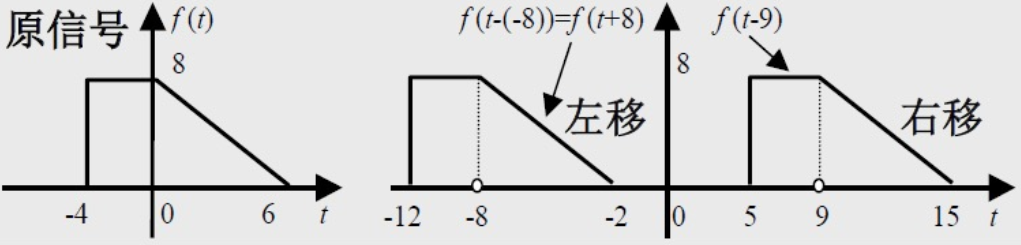
\includegraphics[width=0.5\textwidth]{chap1/img/waveform-translation.png}
        \caption{信号的时移运算}
        \label{fig:waveform-translation}
    \end{figure}
\end{example}

\begin{definition}[反褶运算]
    信号的\bd{反褶运算}是指,将原信号 $f(t)$ 按照纵轴对称翻转过来,
    得到新信号 $f(-t)$。
\end{definition}

\begin{example}
    如图 \ref{fig:waveform-symmetry} 所示,假设有原信号 $f(t)$,
    则其反褶信号为 $f(-t)$。
    \begin{figure}[H]
        \centering
        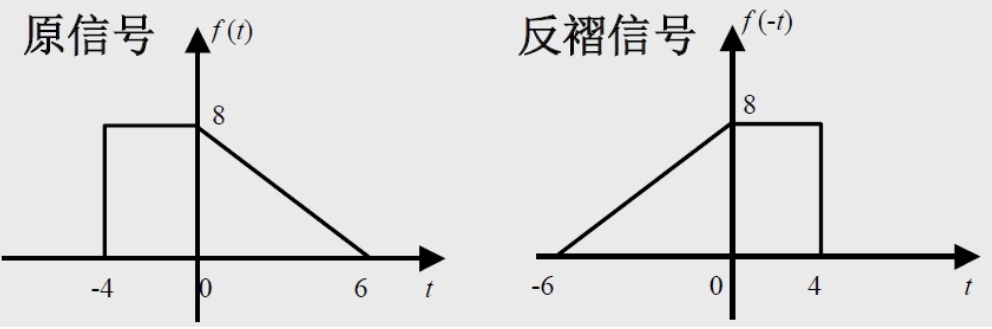
\includegraphics[width=0.5\textwidth]{chap1/img/waveform-symmetry.png}
        \caption{信号的反褶运算}
        \label{fig:waveform-symmetry}
    \end{figure}
\end{example}

\begin{definition}[压扩运算]
    信号的\bd{压扩运算}是指,将原信号 $f(t)$ 沿横轴缩放 $a$ 倍,
    得到新信号 $f(at)$。其中,实参数 $a$ 决定缩放方向和缩放倍数。
    当 $a < 0$ 时,信号需要先进行反褶运算,再进行压扩运算。
    \begin{itemize}
        \item $0 < \abs{a} < 1$ 时,信号在横轴方向上缩小。
        \item $\abs{a} > 1$ 时,信号在横轴方向上放大。
    \end{itemize}
\end{definition}

\begin{example}
    如图 \ref{fig:waveform-scaling} 所示,假设有原信号 $f(t)$,
    则其压扩信号 $f(2t)$ 和 $f(-0.5t)$ 如图所示。
    \begin{figure}[H]
        \centering
        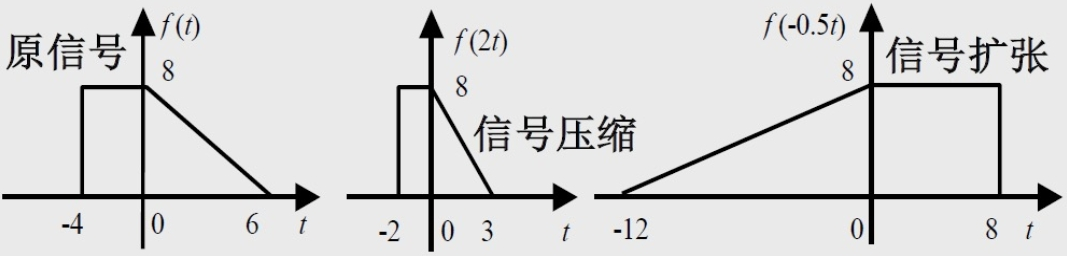
\includegraphics[width=0.5\textwidth]{chap1/img/waveform-scaling.png}
        \caption{信号的压扩运算}
        \label{fig:waveform-scaling}
    \end{figure}
\end{example}

\begin{example}
    已知信号 $f(t)$ 如图 \ref{fig:waveform-exercise-0} 所示,
    请画出 $y(t) = 3f\left(1 - \frac{t}{2}\right) - 1$ 的图形。
    \begin{figure}[H]
        \centering
        \begin{tikzpicture}
            \begin{axis}[
                axis lines = middle,
                xlabel = {$t$},
                ylabel = {$f(t)$},
                ylabel style={at={(rel axis cs:0.4, 1)}, anchor=south},
                xmin = -1.2, xmax = 2.2,
                ymin = -0.2, ymax = 1.2,
                xtick distance = 1,
                ytick distance = 1,
                grid = major,
                grid style = dashed,
                scale only axis,
                width = 8cm,
                height = 3cm,
                axis equal,
            ]
            \addplot[domain=-1.2:-1, samples=100, smooth, blue] {0};
            \addplot[smooth, blue] coordinates {(-1, 0) (-1, 1)};
            \addplot[domain=-1:0, samples=100, smooth, blue] {1};
            \addplot[smooth, blue] coordinates {(0, 1) (0, 0)};
            \addplot[domain=0:1, samples=100, smooth, blue] {x};
            \addplot[domain=1:2, samples=100, smooth, blue] {1};
            \addplot[smooth, blue] coordinates {(2, 1) (2, 0)};
            \addplot[domain=2:2.2, samples=100, smooth, blue] {0};
            \addlegendentry{$f(t)$}
            \node at (axis cs:0,0) [anchor=north west] {O};
            \end{axis}
        \end{tikzpicture}
        \caption{$f(t)$ 的波形描述}
        \label{fig:waveform-exercise-0}
    \end{figure}
\end{example}

\begin{solution}
    首先,对 $f(t)$ 进行时移运算,
    得到 $f\left(1 + t\right)$ 的波形如图 \ref{fig:waveform-exercise-1} 所示。
    \begin{figure}[H]
        \centering
        \begin{tikzpicture}
            \begin{axis}[
                axis lines = middle,
                xlabel = {$t$},
                ylabel = {$f(1 + t)$},
                ylabel style={at={(rel axis cs:0.4, 1)}, anchor=south},
                xmin = -2.2, xmax = 1.2,
                ymin = -0.2, ymax = 1.2,
                xtick distance = 1,
                ytick distance = 1,
                grid = major,
                grid style = dashed,
                scale only axis,
                width = 8cm,
                height = 3cm,
                axis equal,
            ]
            \addplot[domain=-2.2:-2, samples=100, smooth, blue] {0};
            \addplot[smooth, blue] coordinates {(-2, 0) (-2, 1)};
            \addplot[domain=-2:-1, samples=100, smooth, blue] {1};
            \addplot[smooth, blue] coordinates {(-1, 1) (-1, 0)};
            \addplot[domain=-1:0, samples=100, smooth, blue] {1 + x};
            \addplot[domain=0:1, samples=100, smooth, blue] {1};
            \addplot[smooth, blue] coordinates {(1, 1) (1, 0)};
            \addplot[domain=1:1.2, samples=100, smooth, blue] {0};
            \node at (axis cs:0, 0) [anchor=north west] {O};
            \end{axis}
        \end{tikzpicture}
        \caption{$f(1 - t)$ 的波形描述}
        \label{fig:waveform-exercise-1}
    \end{figure}

    其次,对 $f\left(1 + t\right)$ 进行反褶和压扩运算,
    得到 $f\left(1 - \frac{t}{2}\right)$ 的波形如图 \ref{fig:waveform-exercise-2} 所示。
    \begin{figure}[H]
        \centering
        \begin{tikzpicture}
            \begin{axis}[
                axis lines = middle,
                xlabel = {$t$},
                ylabel = {$f\left(1 - \frac{t}{2}\right)$},
                ylabel style={at={(rel axis cs:0.4, 1)}, anchor=south},
                xmin = -2.2, xmax = 4.2,
                ymin = -0.2, ymax = 1.2,
                xtick distance = 1,
                ytick distance = 1,
                grid = major,
                grid style = dashed,
                scale only axis,
                width = 8cm,
                height = 3cm,
                axis equal,
            ]
            \addplot[domain=-2.2:-2, samples=100, smooth, blue] {0};
            \addplot[smooth, blue] coordinates {(-2, 0) (-2, 1)};
            \addplot[domain=-2:0, samples=100, smooth, blue] {1};
            \addplot[domain=0:2, samples=100, smooth, blue] {1 - 1/2 * x};
            \addplot[smooth, blue] coordinates {(2, 0) (2, 1)};
            \addplot[domain=2:4, samples=100, smooth, blue] {1};
            \addplot[smooth, blue] coordinates {(4, 1) (4, 0)};
            \addplot[domain=4:4.2, samples=100, smooth, blue] {0};
            \node at (axis cs:0, 0) [anchor=north west] {O};
            \end{axis}
        \end{tikzpicture}
        \caption{$f\left(1 - \frac{t}{2}\right)$ 的波形描述}
        \label{fig:waveform-exercise-2}
    \end{figure}
    
    再次,对 $f\left(1 - \frac{t}{2}\right)$ 进行纵轴方向的缩放和平移,
    得到 $3f\left(1 - \frac{t}{2}\right) - 1$ 的波形如图 \ref{fig:waveform-exercise-3} 所示。
    \begin{figure}[H]
        \centering
        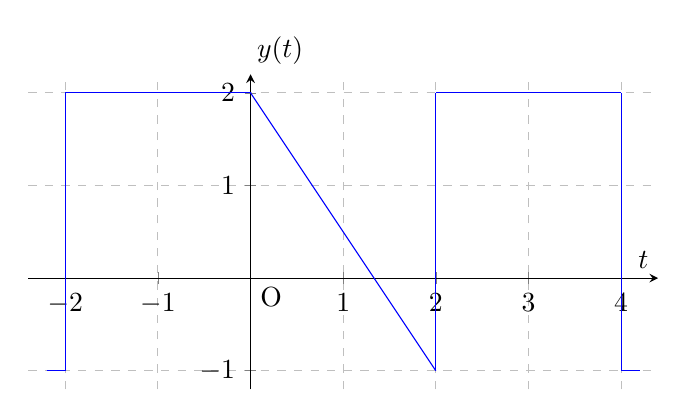
\begin{tikzpicture}
            \begin{axis}[
                axis lines = middle,
                xlabel = {$t$},
                ylabel = {$y(t)$},
                ylabel style={at={(rel axis cs:0.4,1)}, anchor=south},
                xmin = -2.2, xmax = 4.2,
                ymin = -1.2, ymax = 2.2,
                xtick distance = 1,
                ytick distance = 1,
                grid = major,
                grid style = dashed,
                scale only axis,
                width = 8cm,
                height = 4cm,
                axis equal,
            ]
            \addplot[domain=-2.2:-2, samples=100, smooth, blue] {-1};
            \addplot[smooth, blue] coordinates {(-2, -1) (-2, 2)};
            \addplot[domain=-2:0, samples=100, smooth, blue] {2};
            \addplot[domain=0:2, samples=100, smooth, blue] {2 - 3/2 * x};
            \addplot[smooth, blue] coordinates {(2, -1) (2, 2)};
            \addplot[domain=2:4, samples=100, smooth, blue] {2};
            \addplot[smooth, blue] coordinates {(4, 2) (4, -1)};
            \addplot[domain=4:4.2, samples=100, smooth, blue] {-1};
            \node at (axis cs:0, 0) [anchor=north west] {O};
            \end{axis}
        \end{tikzpicture}
        \caption{$3f\left(1 - \frac{t}{2}\right)-1$ 的波形描述}
        \label{fig:waveform-exercise-3}
    \end{figure}

\end{solution}

\begin{remark}
    假设有原信号 $y = f(t)$,我们需要画出 $y = Af(\omega t + \varphi) + B$ 的图像时,
    可以按照以下步骤进行:
    \begin{enumerate}
        \item 画出 $y = f(t + \varphi)$ 的图像。
        \item 画出 $y = f(\abs{\omega} t + \varphi)$ 的图像。若 $\omega < 0$ 则再进行反褶(关于 $y$ 轴进行对称)。
        \item 画出 $y = Af(\omega t + \varphi) + B$ 的图像。
    \end{enumerate}
\end{remark}

\begin{note}
    记得标注坐标轴的原点、标注横轴和纵轴的刻度和标识。记得画 $f(t) = 0$ 对应的 $y(t)$ 图像(在上例中,
    对应的是 $(-\infty, -2]$ 和 $[4, +\infty)$ 上的图像 $y = -1$。
\end{note}

\subsubsection{微分与积分运算}

\begin{definition}[信号的能量与功率]
    信号的\bd{能量}和\bd{功率}是描述信号强度的两个重要指标。
    \begin{itemize}
        \item 当信号为连续信号时,信号的\bd{能量}定义为
            \begin{align*}
                E = \int_{-\infty}^{+\infty}\abs{f(t)}^2\D{t},
            \end{align*}
            信号的\bd{功率}定义为
            \begin{align*}
                P = \lim_{T \to +\infty}\frac{1}{2T}\int_{-T}^{T}\abs{f(t)}^2\D{t}.
            \end{align*}
        \item 当信号为离散信号时,信号的\bd{能量}定义为
            \begin{align*}
                E = \sum_{n = -\infty}^{+\infty}\abs{f(n)}^2,
            \end{align*}
            信号的\bd{功率}定义为
            \begin{align*}
                P = \lim_{N \to +\infty}\frac{1}{2N + 1}\sum_{n = -N}^{N}\abs{f(n)}^2.
            \end{align*}
    \end{itemize}
\end{definition}

\begin{definition}[能量信号与功率信号]
    如果信号的能量是有限的,则称为能量有限信号,简称\bd{能量信号}。
    如果信号的功率是有限的,则称为功率有限信号,简称\bd{功率信号}。
\end{definition}

\subsubsection{卷积运算}

\begin{definition}
    设 $f(t), g(t)$ 为两个连续时间信号函数,则它们的\bd{卷积}定义为
    \begin{align*}
        (f * g)(t) = f(t) * g(t) = \int_{-\infty}^{+\infty}f(t - \tau)g(\tau)\D{\tau}.
    \end{align*}

    若 $f(n), g(n)$ 为两个离散时间信号函数,$f, g$ 是 $\set{Z}$ 上的离散序列,
    则它们的\bd{卷积}定义为
    \begin{align*}
        (f * g)(n) = f(n) * g(n) = \sum_{k = -\infty}^{+\infty}f(n - k)g(k).
    \end{align*}
\end{definition}

\begin{remark}
    两个信号的卷积是否存在是有条件的:
    \begin{itemize}
        \item $f, g$ 均为可积函数。
        \item $f, g$ 卷积运算的结果是有界的。
    \end{itemize}
\end{remark}

\begin{note}
    一个信号的反褶信号在 $t$ 轴滑动过程中,
    它与另外一个信号重合部分相乘得到的新信号的面积
    随 $t$ 的变化曲线,就是所求的两个信号的卷积的波形,如图 \ref{fig:convolution-explanation} 所示。
    \begin{figure}[H]
        \centering
        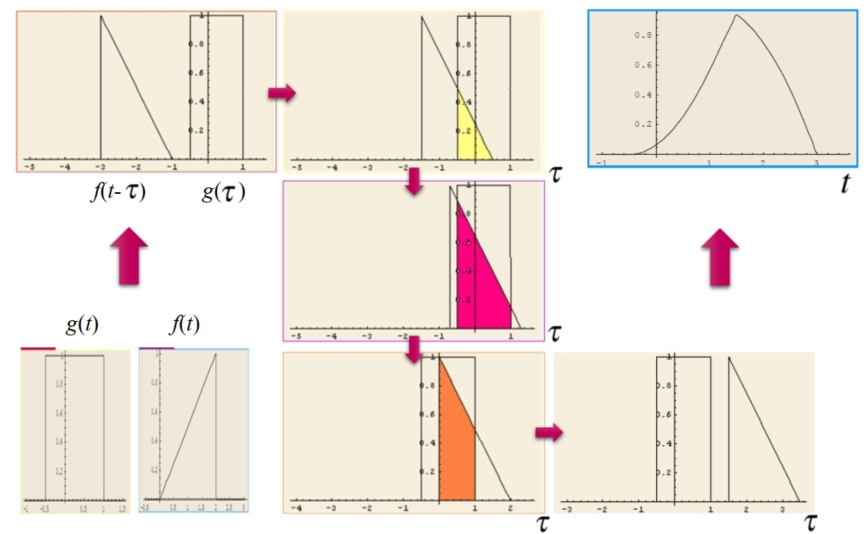
\includegraphics[width=0.5\textwidth]{chap1/img/convolution-explanation.png}
        \caption{卷积运算的解释}
        \label{fig:convolution-explanation}
    \end{figure}
    需要注意的是,卷积不是求图形相交部分的面积,而是求相乘结果的函数的面积。
\end{note}

\begin{property}[卷积运算的交换律]
    卷积运算具有交换律:
    \begin{align*}
        f_1 * f_2 = f_2 * f_1.
    \end{align*}
\end{property}

卷积运算的交换律可以通过变换积分变量的方式来证明。

\begin{proof}
    \begin{align*}
        (f_1 * f_2)(t) & = \int_{-\infty}^{+\infty}f_1(t - a)f_2(a)\D{a} \\
        & = \int_{+\infty}^{-\infty}f_1(b)f_2(t - b)\cdot (-\D{b}) \quad (b = t - a) \\
        & = \int_{-\infty}^{+\infty}f_2(t - b)f_1(b)\D{b} \\
        & = (f_2 * f_1)(t).
    \end{align*}
\end{proof}

\begin{property}[卷积运算的分配律]
    卷积运算具有分配律:
    \begin{align*}
        f_1 * (f_2 + f_3) = f_1 * f_2 + f_1 * f_3.
    \end{align*}
    卷积运算的分配律通常用于并联系统的分析。
\end{property}

卷积运算的分配率可以利用积分运算的线性性来证明。

\begin{proof}
    \begin{align*}
        (f_1 * (f_2 + f_3))(t) & = \int_{-\infty}^{+\infty}f_1(t - a)(f_2(a) + f_3(a))\D{a} \\
        & = \int_{-\infty}^{+\infty}f_1(t - a)f_2(a)\D{a} + \int_{-\infty}^{+\infty}f_1(t - a)f_3(a)\D{a} \\
        & = (f_1 * f_2)(t) + (f_1 * f_3)(t) \\
        & = (f_1 * f_2 + f_1 * f_3)(t).
    \end{align*}
\end{proof}

\begin{property}[卷积运算的结合律]
    卷积运算具有结合律:
    \begin{align*}
        (f_1 * f_2) * f_3 = f_1 * (f_2 * f_3).
    \end{align*}
    卷积运算的结合律通常用于串联系统的分析。
\end{property}

\begin{proof}
    \begin{align*}
        ((f_1 * f_2) * f_3)(t) & = \int_{-\infty}^{+\infty}\left[\int_{-\infty}^{+\infty}f_1(a) f_2(b - a)\D{a}\right]f_3(t - b)\D{b} \\
        & = \int_{-\infty}^{+\infty}f_1(a)\left[\int_{-\infty}^{+\infty}f_2(b - a)f_3(t - b)\D{b}\right]\D{a} \\
        & = \int_{-\infty}^{+\infty}f_1(a)\left[\int_{-\infty}^{+\infty}f_2(c)f_3(t - a - c)\D{c}\right]\D{a}, \quad (c = b - a) \\
        & = \int_{-\infty}^{+\infty}f_1(a)(f_2 * f_3)(t - a)\D{a} \\
        & = (f_1 * (f_2 * f_3))(t).
    \end{align*}
\end{proof}

\begin{property}[卷积的微分性质]
    卷积的微分满足以下性质:两个信号卷积的微分等于其中任一信号的微分与另一信号的卷积,即
    \begin{align*}
        \frac{\D}{\D{t}}\left[f_1(t) * f_2(t)\right]
        = f_1(t) * \frac{\D}{\D{t}}\left[f_2(t)\right]
        = \frac{\D}{\D{t}}\left[f_1(t)\right] * f_2(t),
    \end{align*}
    其中 $f_1, f_2$ 为  $\set{R}$ 上连续可导函数。
\end{property}

\begin{proof}
    \begin{align*}
        \frac{\D}{\D{t}}\left[f_1(t) * f_2(t)\right]
        & = \frac{\D}{\D{t}}\left[\int_{-\infty}^{+\infty}f_1(a) \cdot f_2(t - a)\D{a}\right] \\
        & = \int_{-\infty}^{+\infty}f_1(a) \cdot \frac{\D}{\D{t}}\left[f_2(t - a)\right]\D{a}.
    \end{align*}
    记 $g(t) = \frac{\D}{\D{t}}\left[f_2(t)\right]$,则 $g(t - a) = \frac{\D}{\D{t}}\left[f_2(t - a)\right]$。因此
    \begin{align*}
        \int_{-\infty}^{+\infty}f_1(a) \cdot \frac{\D}{\D{t}}\left[f_2(t - a)\right]\D{a}
        = \int_{-\infty}^{+\infty}f_1(a) \cdot g(t - a)\D{a}
        = f_1(t) * g(t)
        = f_1(t) * \frac{\D}{\D{t}}\left[f_2(t)\right].
    \end{align*}
    同理,由卷积运算的交换律可以证明 $\frac{\D}{\D{t}}\left[f_1(t) * f_2(t)\right] = \frac{\D}{\D{t}}\left[f_1(t)\right] * f_2(t)$。
    因此,命题得证。
\end{proof}

\begin{property}[卷积的积分性质]
    卷积的积分满足以下性质:两个信号卷积的积分等于其中任一信号的积分与另一信号的卷积,即
    \begin{align*}
        \int_{-\infty}^{t}(f_1 * f_2)(\lambda)\D{\lambda}
        = f_1(t) * \left(\int_{-\infty}^{t}f_2(\lambda)\D{\lambda}\right)
        = \left(\int_{-\infty}^{t}f_1(\lambda)\D{\lambda}\right) * f_2(t),
    \end{align*}
    其中 $f_1, f_2$ 为  $\set{R}$ 上连续可导函数。
\end{property}

\begin{proof}
    \begin{align*}
        \int_{-\infty}^{t}(f_1 * f_2)(\lambda)\D{\lambda}
        & = \int_{-\infty}^{t}\left[\int_{-\infty}^{+\infty}f_1(a)f_2(\lambda - a)\D{a}\right]\D{\lambda} \\
        & = \int_{-\infty}^{+\infty}f_1(a)\left[\int_{-\infty}^{t}f_2(\lambda - a)\D{\lambda}\right]\D{a}.
    \end{align*}
    记 $g(t) = \int_{-\infty}^{t}f_2(\lambda)\D{\lambda}$,
    则 $g(t - a) = \int_{-\infty}^{t - a}f_2(\lambda')\D{\lambda'} = \int_{-\infty}^{t}f_2(\lambda - a)\D{\lambda}, \lambda = \lambda' + a$。因此
    \begin{align*}
        \int_{-\infty}^{+\infty}f_1(a)\left[\int_{-\infty}^{t}f_2(\lambda - a)\D{\lambda}\right]\D{a}
        = \int_{-\infty}^{+\infty}f_1(a)g(t - a)\D{a}
        = f_1(t) * g(t)
        = f_1(t) * \left(\int_{-\infty}^{t}f_2(\lambda)\D{\lambda}\right).
    \end{align*}
    同理,由卷积运算的交换律可以证明 $\int_{-\infty}^{t}(f_1 * f_2)(\lambda)\D{\lambda} = \left(\int_{-\infty}^{t}f_1(\lambda)\D{\lambda}\right) * f_2(t)$。
    因此,命题得证。
    
\end{proof}

\begin{corollary}
    设 $f_1, f_2$ 为 $\set{R}$ 上的 $n$ 次可微函数,则
    \begin{align*}
        (f_1 * f_2)^{(n)}(t) = f_1^{(m)}(t) * f_2^{(n - m)}(t), \quad m = 0, 1, \cdots, n.
    \end{align*}
    特别地,当 $n < 0$ 时,记 $f^{(n)}(t)$ 表示对 $f(t)$ 进行 $n$ 次积分运算,则
    \begin{align*}
        (f_1 * f_2)^{(n)}(t) = f_1^{(m)}(t) * f_2^{(n - m)}(t), \quad m = n, n + 1, \cdots, 0.
    \end{align*}
    也就是说,卷积运算的求导次数可以被分配到两个函数上,分别求导后再进行卷积运算;
    积分运算的次数也可以被分配到两个函数上,分别积分后再进行卷积运算。
\end{corollary}

\begin{proof}
    只证明 $n > 0$ 的情况,$n < 0$ 的情况的证明与之类似。使用数学归纳法证明。
    
    当 $n = 1$ 时,由卷积的微分性质即可得证。假设 $n = k$ 时结论成立,即
    \begin{align*}
        (f_1 * f_2)^{(k)}(t) = f_1^{(m)}(t) * f_2^{(k - m)}(t), \quad m = 0, 1, \cdots, k.
    \end{align*}
    当 $n = k + 1$ 时,有
    \begin{align*}
        (f_1 * f_2)^{(k + 1)}(t) & = \frac{\D}{\D{t}}\left[(f_1 * f_2)^{(k)}(t)\right] \\
        & = \frac{\D}{\D{t}}\left[f_1^{(m)}(t) * f_2^{(k - m)}(t)\right] \\
        & = f_1^{(m + 1)}(t) * f_2^{(k - m)}(t) \\
        & = f_1^{(m)}(t) * f_2^{(k - m + 1)}(t).
    \end{align*}
    因此,由数学归纳法可知,对于任意的 $n \ge 0$,结论均成立。
\end{proof}

\subsubsection{相关运算}

\begin{definition}
    两个信号的\bd{相关运算}定义为
    \begin{align*}
        R_{f_1, f_2}(t)
        = R(f_1(t), f_2(t))
        = \int_{-\infty}^{+\infty}f_1(\tau)f_2^*(\tau - t)\D{\tau}
        = \int_{-\infty}^{+\infty}f_1(\tau + t)f_2^*(\tau)\D{\tau}.
    \end{align*}
\end{definition}

\begin{remark}
    相关运算和卷积运算有一定的联系:$R_{f_1, f_2}(t) = f_1(t) * f_2^*(-t)$,
    但也有一定的区别:相关运算中的第二个信号\bd{不需要反褶},但\bd{需要取共轭}。
\end{remark}

\begin{property}
    信号的相关运算与顺序有关。考虑 $R_{f_2, f_2}(t)$:
    \begin{align*}
        R_{f_2, f_1}(t) = R(f_2(t), f_1(t)) = \int_{-\infty}^{+\infty}f_2(\tau)f_1^*(\tau - t)\D{\tau}.
    \end{align*}
    对比 $R_{f_1, f_2}(t)$,可以发现
    \begin{align*}
        R_{f_2, f_1}(t) & = \int_{-\infty}^{+\infty}f_1(a)f_2^*(a - t)\D{a} \\
        & = \left[\int_{-\infty}^{+\infty}f_1^*(a)f_2(a - t)\D{a}\right]^* \\
        & = R_{f_1, f_2}^*(-t).
    \end{align*}
\end{property}

\begin{note}
    \begin{align*}
        f_1(t) * f_2(t) & = \int_{-\infty}^{+\infty}f_1(t - a)f_2(a)\D{a}, \\
        f_1(-t) * f_2(t) & = \int_{-\infty}^{+\infty}f_1(a - t)f_2(a)\D{a} \\
        & \neq \int_{-\infty}^{+\infty}f_1(-t - a)f_2(a)\D{a}.
    \end{align*}
    一个比较容易的方法,是记 $g(t) = f_1(-t)$,
    这样 $g(t) * f_2(t) = \int_{-\infty}^{+\infty}g(t - a)f_2(a)\D{a} = \int_{-\infty}^{+\infty}f_1(a - t)f_2(a)\D{a}$,
    就不会记错了。
\end{note}

\begin{example}[自相关运算]
    自相关运算是指函数自己与自己求相关。用自相关函数可以检测准周期信号的准周期,
    如图 \ref{fig:self-relation} 所示。
    \begin{figure}[H]
        \centering
        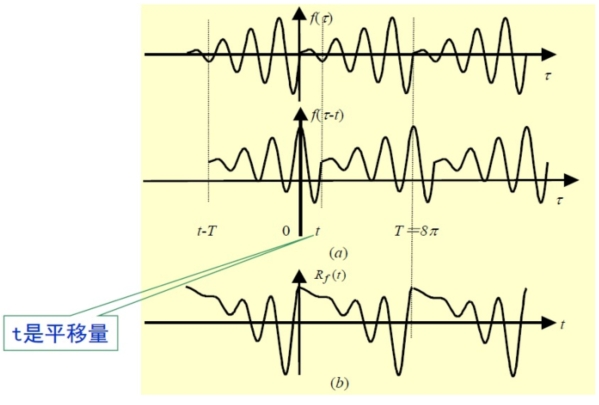
\includegraphics[width=0.5\textwidth]{chap1/img/self-relation.png}
        \caption{函数的自相关运算}
        \label{fig:self-relation}
    \end{figure}
\end{example}

\begin{example}[卷积的物理意义]
    设 $g(x, y)$ 表示图像,$f(x, y)$ 表示卷积核。则如图 \ref{fig:graph-convolution-example-1} 和
    图 \ref{fig:graph-convolution-example-2} 所示,
    \begin{figure}[H]
        \centering
        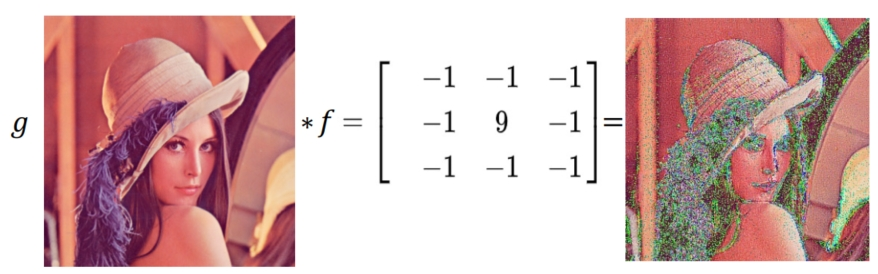
\includegraphics[width=0.5\textwidth]{chap1/img/graph-convolution-example-1.png}
        \caption{卷积的物理意义(1)}
        \label{fig:graph-convolution-example-1}
    \end{figure}
    为何``积''?``积''的过程中,我们得到了一个叠加值,我们通过定义 $f$,使得叠加值包含图像的特定信息,例如边缘信息,平滑处理。
    \begin{figure}[H]
        \centering
        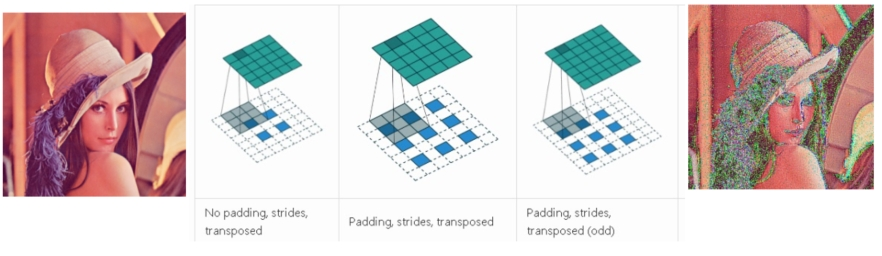
\includegraphics[width=0.5\textwidth]{chap1/img/graph-convolution-example-2.png}
        \caption{卷积的物理意义(2)}
        \label{fig:graph-convolution-example-2}
    \end{figure}
\end{example}

\begin{note}
    卷积的定义中,为何要对 $f$ 做反褶?为了数学上的便利性,反褶后卷积可以满足交换律;
    另一方面,在后续的学习中,我们会发现时域的卷积在频域上有很简洁的形式。
\end{note}

\subsection{奇异信号}

\subsubsection{单位斜变信号}

\begin{definition}[单位斜变信号]
    \bd{单位斜变信号}的数学表达式为
    \begin{align*}
        R(t) = \begin{cases}
            0, & t < 0, \\
            t, & t \ge 0.
        \end{cases}
    \end{align*}
    信号图像如图 \ref{fig:ramp-signal} 所示。
    \begin{figure}[H]
        \centering
        \begin{tikzpicture}
            \begin{axis}[
                axis lines = middle,
                xlabel = {$t$},
                ylabel = {$R(t)$},
                ylabel style={at={(rel axis cs:0.4, 1)}, anchor=south},
                xmin = -1.2, xmax = 2.2,
                ymin = -0.2, ymax = 2.2,
                xtick distance = 1,
                ytick distance = 1,
                grid = major,
                grid style = dashed,
                scale only axis,
                width = 8cm,
                height = 5cm,
                axis equal,
            ]
            \addplot[domain=-1.2:0, samples=100, smooth, blue] {0};
            \addplot[domain=0:2.2, samples=100, smooth, blue] {x};
            \node at (axis cs:0, 0) [anchor=north west] {O};
            \end{axis}
        \end{tikzpicture}
        \caption{单位斜变信号}
        \label{fig:ramp-signal}
    \end{figure}
\end{definition}

\begin{definition}[截顶的单位斜变信号]
    \bd{截顶的单位斜变信号}的数学表达式为
    \begin{align*}
        R_{\tau}(t) = \begin{cases}
            0, & t < 0, \\
            t, & 0 \le t \le \tau, \\
            \tau, & t > \tau.
        \end{cases}
    \end{align*}
    信号图像如图 \ref{fig:truncated-ramp-signal} 所示。
    \begin{figure}[H]
        \centering
        \begin{tikzpicture}
            \begin{axis}[
                axis lines = middle,
                xlabel = {$t$},
                ylabel = {$R_{\tau}(t)$},
                ylabel style={at={(rel axis cs:0.4, 1)}, anchor=south},
                xmin = -1.2, xmax = 1.5,
                ymin = -0.2, ymax = 1.5,
                xtick distance = 1,
                ytick distance = 1,
                grid = major,
                grid style = dashed,
                scale only axis,
                width = 8cm,
                height = 6cm,
                axis equal,
            ]
            \addplot[domain=-1.2:0, samples=100, smooth, blue] {0};
            \addplot[domain=0:1.3, samples=100, smooth, blue] {x};
            \addplot[domain=1.3:2.2, samples=100, smooth, blue] {1.3};
            \addplot[smooth, red, dashed] coordinates {(0, 1.3) (1.3, 1.3)};
            \addplot[smooth, red, dashed] coordinates {(1.3, 0) (1.3, 1.3)};
            \node at (axis cs:0, 0) [anchor=north west] {O};
            \node at (axis cs:0, 1.3) [anchor = east] {$\tau$};
            \node at (axis cs:1.3, 0) [anchor = north] {$\tau$};
            \end{axis}
        \end{tikzpicture}
        \caption{截顶的单位斜变信号}
        \label{fig:truncated-ramp-signal}
    \end{figure}
\end{definition}

\subsubsection{单位阶跃信号}

\begin{definition}[单位阶跃信号]
    \bd{单位阶跃信号}的数学表达式为
    \begin{align*}
        u(t) = \begin{cases}
            0, & t < 0, \\
            1, & t \ge 0.
        \end{cases}
    \end{align*}
    信号图像如图 \ref{fig:step-signal} 所示。
    \begin{figure}[H]
        \centering
        \begin{tikzpicture}
            \begin{axis}[
                axis lines = middle,
                xlabel = {$t$},
                ylabel = {$u(t)$},
                ylabel style={at={(rel axis cs:0.1, 1)}, anchor=south},
                xmin = -0.2, xmax = 2.2,
                ymin = -0.2, ymax = 1.2,
                xtick distance = 1,
                ytick distance = 1,
                grid = major,
                grid style = dashed,
                scale only axis,
                width = 8cm,
                height = 5cm,
                axis equal,
            ]
            \addplot[domain=-1.2:0, samples=100, smooth, blue] {0};
            \addplot[domain=0:2.2, samples=100, smooth, blue] {1};
            \node at (axis cs:0, 0) [anchor=north west] {O};
            \end{axis}
        \end{tikzpicture}
        \caption{单位阶跃信号}
        \label{fig:step-signal}
    \end{figure}
\end{definition}

\begin{property}[单位阶跃信号与单位斜变信号的关系]
    单位斜变信号是单位阶跃信号的积分,即
    \begin{align*}
        R(t) = \int_{-\infty}^{t}u(\tau)\D{\tau}.
    \end{align*}
    单位阶跃信号是单位斜变信号的微分,即
    \begin{align*}
        u(t) = \frac{\D{R(t)}}{\D{t}}.
    \end{align*}
\end{property}

\subsubsection{单位矩形脉冲信号}

\begin{definition}[单位矩形脉冲信号]
    \bd{单位矩形脉冲信号}的数学表达式为
    \begin{align*}
        G_{\tau}(t) = \begin{cases}
            0, & \abs{t} \le \frac{\tau}{2}, \\
            1, & \abs{t} > \frac{\tau}{2}.
        \end{cases}
    \end{align*}
    信号图像如图 \ref{fig:rectangular-pulse-signal} 所示。
    \begin{figure}[H]
        \centering
        \begin{tikzpicture}
            \begin{axis}[
                axis lines = middle,
                xlabel = {$t$},
                ylabel = {$G_{\tau}(t)$},
                ylabel style={at={(rel axis cs:0.5, 1)}, anchor=south},
                xmin = -2.2, xmax = 2.2,
                ymin = -0.2, ymax = 1.2,
                xtick distance = 1,
                ytick distance = 1,
                grid = major,
                grid style = dashed,
                scale only axis,
                width = 8cm,
                height = 5cm,
                axis equal,
            ]
            \addplot[domain=-2.2:-1.3, samples=100, smooth, blue] {0};
            \addplot[domain=-1.3:1.3, samples=100, smooth, blue] {1};
            \addplot[domain=1.3:2.2, samples=100, smooth, blue] {0};
            \addplot[smooth, blue] coordinates {(-1.3, 0) (-1.3, 1)};
            \addplot[smooth, blue] coordinates {(1.3, 1) (1.3, 0)};
            \node at (axis cs:0, 0) [anchor=north west] {O};
            \node at (axis cs:-1.3, 0) [anchor = north] {$-\frac{\tau}{2}$};
            \node at (axis cs:1.3, 0) [anchor = north] {$\frac{\tau}{2}$};
            \end{axis}
        \end{tikzpicture}
        \caption{单位矩形脉冲信号}
        \label{fig:rectangular-pulse-signal}
    \end{figure}
    其中,\bd{脉高}是指脉冲信号的高度,\bd{脉宽}是指脉冲信号的宽度。
\end{definition}

\begin{property}[单位矩形脉冲信号与单位阶跃信号的关系]
    单位矩形脉冲信号是两个单位阶跃信号的差,即
    \begin{align*}
        G_{\tau}(t) = u\left(t + \frac{\tau}{2}\right) - u\left(t - \frac{\tau}{2}\right).
    \end{align*}
\end{property}

\begin{remark}
    不必再用分段的形式来表示信号,可以使用矩形脉冲信号来表示。
    其他信号与矩形脉冲信号相乘时,只有在矩形脉冲信号对应的区间内,
    其他信号的信息才被保留下来,其余范围都是零。

    用矩形脉冲信号和乘法运算,可以截取信号的特定区间片段。
    所以,单位矩形脉冲信号也被称为``窗函数''。如图 \ref{fig:rectangular-pulse-signal-example} 所示。
    \begin{figure}[H]
        \centering
        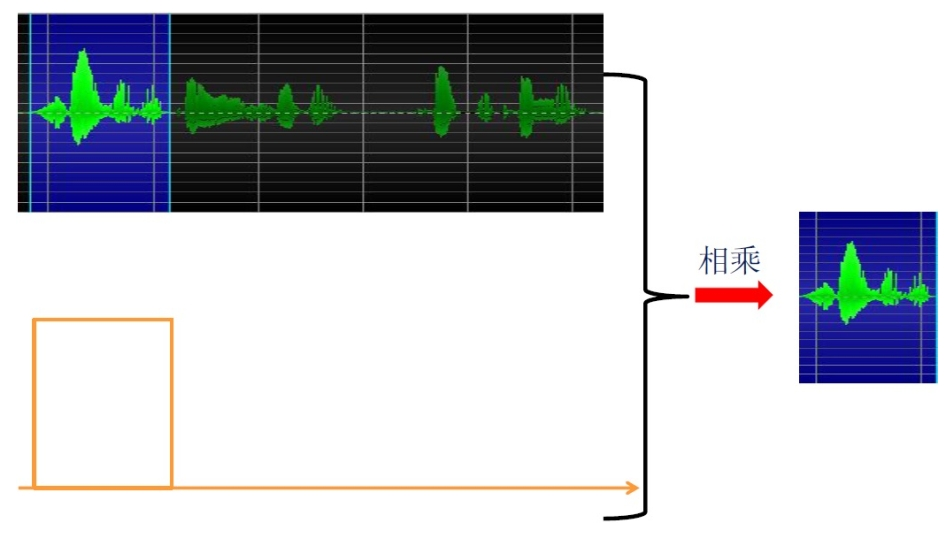
\includegraphics[width=0.5\textwidth]{chap1/img/rectangular-pulse-signal-example.png}
        \caption{窗函数的截取功能}
        \label{fig:rectangular-pulse-signal-example}
    \end{figure}
\end{remark}

\subsubsection{符号函数信号}

\begin{definition}[符号函数信号]
    \bd{符号函数信号}的数学表达式为
    \begin{align*}
        \sgn(t) = \begin{cases}
            -1, & t < 0, \\
            0, & t = 0, \\
            1, & t > 0.
        \end{cases}
    \end{align*}
    信号图像如图 \ref{fig:sign-signal} 所示。
    \begin{figure}[H]
        \centering
        \begin{tikzpicture}
            \begin{axis}[
                axis lines = middle,
                xlabel = {$t$},
                ylabel = {$\sgn(t)$},
                ylabel style={at={(rel axis cs:0.5, 1)}, anchor=south},
                xmin = -2.2, xmax = 2.2,
                ymin = -1.2, ymax = 1.2,
                xtick distance = 1,
                ytick distance = 1,
                grid = major,
                grid style = dashed,
                scale only axis,
                width = 8cm,
                height = 5cm,
                axis equal,
            ]
            \addplot[domain=-2.2:0, samples=100, smooth, blue] {-1};
            \addplot[domain=0:2.2, samples=100, smooth, blue] {1};
            \addplot[smooth, blue] coordinates {(0, -1) (0, 1)};
            \node at (axis cs:0, 0) [anchor=north west] {O};
            \end{axis}
        \end{tikzpicture}
        \caption{符号函数信号}
        \label{fig:sign-signal}
    \end{figure}
    符号函数信号通常用于表示自变量的符号特性。
\end{definition}

\begin{property}[符号函数信号与单位阶跃信号的关系]
    由 $\sgn(t) + 1 = 2u(t)$ 可得,
    \begin{align*}
        \sgn(t) = 2u(t) - 1.
    \end{align*}
\end{property}

\subsubsection{单位冲激信号}

\begin{definition}[单位冲激信号的狄拉克定义式]
    设冲激信号有一个总的冲激强度,它在整个时间域上的积分等于该强度值,
    而在除冲激点之外的其他点的函数取值为零。
    定义\bd{单位冲激信号}$\delta(t)$ 为满足以下条件的信号:
    \begin{align*}
        \begin{cases}
            \int_{-\infty}^{+\infty}\delta(t)\D{t} = 1, \\
            \delta(t) = 0 \quad (t \neq t_0).
        \end{cases}
    \end{align*}
    这也被称为 $\delta(t)$ 的狄拉克定义式。
    更一般地,可以定义冲激点在 $t_0$,强度为 $E$ 的冲激信号为
    \begin{align*}
        \delta_{E, t_0}(t) = E \cdot \delta(t - t_0),
    \end{align*}
    它满足
    \begin{align*}
        \begin{cases}
            \int_{-\infty}^{+\infty}\delta_{E, t_0}(t)\D{t} = E, \\
            \delta_{E, t_0}(t) = 0 \quad (t \neq t_0).
        \end{cases}
    \end{align*}

    信号图像如图 \ref{fig:impulse-signal} 所示。
    在冲激点处画一条带箭头的线,线的方向和长度与冲激强度的符号和大小一致。
    \begin{figure}[H]
        \centering
        \begin{tikzpicture}
            \begin{axis}[
                axis lines = middle,
                xlabel = {$t$},
                ylabel = {$\delta(t)$},
                ylabel style={at={(rel axis cs:0.5, 1)}, anchor=south},
                xmin = -0.2, xmax = 2.2,
                ymin = -0.2, ymax = 2.2,
                xtick distance = 1,
                ytick distance = 1,
                grid = major,
                grid style = dashed,
                scale only axis,
                width = 6cm,
                height = 5cm,
                axis equal,
            ]
            \draw[-stealth, blue] (axis cs:1.3, 0) -- (axis cs:1.3, 1.5);
            \node at (axis cs:0, 0) [anchor=north west] {O};
            \node at (axis cs:1.3, 0) [anchor=north] {$t_0$};
            \node at (axis cs:1.3, 1.5) [anchor=west] {$(E)$};
            \end{axis}
        \end{tikzpicture}
        \caption{单位冲激信号}
        \label{fig:impulse-signal}
    \end{figure}

    单位冲激信号通常用于描述自然界中那些发生后持续时间很短的现象。
\end{definition}

\begin{definition}[单位冲激信号的极限定义式]
    设 $G_{\tau}(t)$ 是一个单位矩形脉冲信号,其脉宽为 $\tau$,则
    \begin{align*}
        \delta(t) = \lim_{\tau \to 0}\frac{G_{\tau}(t)}{\tau},
    \end{align*}
    即单位冲激信号是单位矩形脉冲信号的极限。
\end{definition}

\begin{remark}
    更一般地,设位于 $[-\frac{\tau}{2}, \frac{\tau}{2}]$ 上的
    信号 $f_{\tau}(t)$ 的脉冲宽度为 $\tau$,若能保证
    \begin{align*}
        \int_{-\frac{\tau}{2}}^{\frac{\tau}{2}}f_{\tau}(t)\D{t} = 1, \quad \forall \tau > 0,
    \end{align*}
    即始终保持单位面积,则
    \begin{align*}
        \delta(t) = \lim_{\tau \to 0}f_{\tau}(t),
    \end{align*}
    即单位冲激信号是信号 $f_{\tau}(t)$ 的极限。$f_{\tau}(t)$ 可以是矩形脉冲、三角脉冲等。
\end{remark}

\begin{property}[冲激函数的搬移抽样特性]
    对于任意的信号 $f(t)$ 而言,都有 $f(t) * \delta(t) = f(t)$。
    更一般地,一个函数与单位冲激函数的卷积,等价于把该函数平移到
    单位冲激函数的冲激点位置,即
    \begin{align*}
        f(t) * \delta(t - t_0) = f(t - t_0),
    \end{align*}
    运算前后的信号如图 \ref{fig:impulse-signal-convolution-translation} 所示。
    \begin{figure}[H]
        \centering
        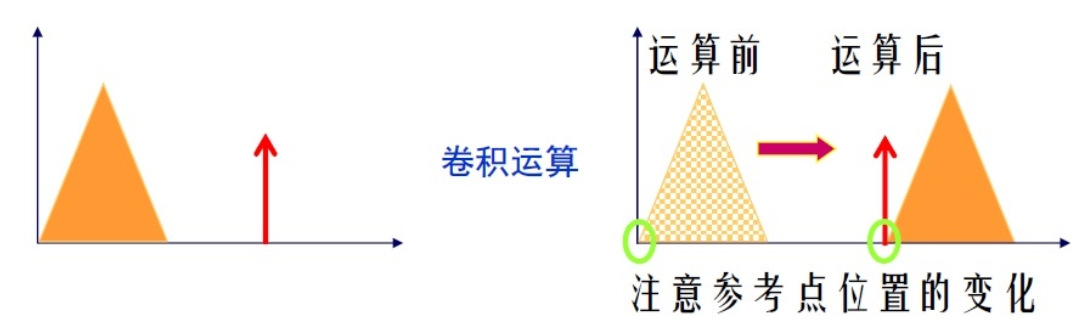
\includegraphics[width=0.5\textwidth]{chap1/img/impulse-signal-convolution-translation.png}
        \caption{冲激函数的搬移抽样特性}
        \label{fig:impulse-signal-convolution-translation}
    \end{figure}
\end{property}

\begin{proof}
    \begin{align*}
        f(t) * \delta(t - t_0) = \int_{-\infty}^{+\infty}f(a)\delta(t - t_0 - a)\D{a},
    \end{align*}
    而 $\delta(t - t_0 - a)$ 只有在 $a = t - t_0$ 时非零。因此
    \begin{align*}
        f(t) * \delta(t - t_0) & = \int_{-\infty}^{+\infty}f(t - t_0)\delta(t - t_0 - a)\D{a} \\
        & = f(t - t_0)\int_{-\infty}^{+\infty}\delta(t - t_0 - a)\D{a} \\
        & = f(t - t_0).
    \end{align*}
\end{proof}

\begin{property}[从函数到值的映射关系]
    冲激函数能从检验函数中筛选出零点处的函数值。对于任意的函数 $f(t)$,有
    \begin{align*}
        \int_{-\infty}^{+\infty}f(t)\delta(t)\D{t} = f(0).
    \end{align*}

    上式只是借用了积分的形式,表达的意思是:冲激函数对测试函数分配(或赋予)一个数的过程,
    所以不能按普通的积分运算来考虑。
    之所以借用积分的形式,是因为它形式上与积分运算的相应性质一致,
    且普通积分运算实际上也是产生一个``值''。
\end{property}

\begin{property}[冲激函数的性质总结]
    冲激函数 $\delta(t)$ 具有以下性质:
    \begin{enumerate}
        \item \nl{(对称性)} $\delta(t)$ 为偶函数,即 $\delta(t) = \delta(-t)$。
        \item \nl{(时域压扩性)} $\delta(at) = \frac{1}{\abs{a}}\delta(t), a \neq 0$。
        \item \nl{(积分)} 积分值为 $1$ 还是 $0$,取决于积分区间是否包含原点,即:
            \begin{align*}
                \begin{cases}
                    \int_{-\infty}^{t}\delta(\tau)\D{\tau} = 1, & t > 0, \\
                    \int_{-\infty}^{t}\delta(\tau)\D{\tau} = 0, & t < 0.
                \end{cases}
            \end{align*}
            即:$\int_{-\infty}^{t}\delta(\tau)\D{\tau} = u(t)$。
            单位冲激函数的积分是单位阶跃函数。
        \item \nl{(抽样特性)} 也称``筛选特性'',即 $\int_{-\infty}^{+\infty}f(t)\delta(t - t_0)\D{t} = f(t_0)$。
    \end{enumerate}
\end{property}

\begin{example}[抽样信号]
    定义\bd{冲激串信号}为
    \begin{align*}
        \Delta_{T_s}(t) = \sum_{n = -\infty}^{+\infty}\delta(t - n T_s),
    \end{align*}
    其中 $T_s$ 是抽样周期。冲激串信号是很多冲激信号的叠加。假设有信号 $f(t)$,则其对应的抽样信号 $f_s(t)$ 为
    \begin{align*}
        f_s(t) = f(t) \cdot \Delta_{T_s}(t) = \sum_{n = -\infty}^{+\infty}f(nT_s)\delta(t - nT_s).
    \end{align*}
    如图 \ref{fig:sampling-signal} 所示。
    \begin{figure}[H]
        \centering
        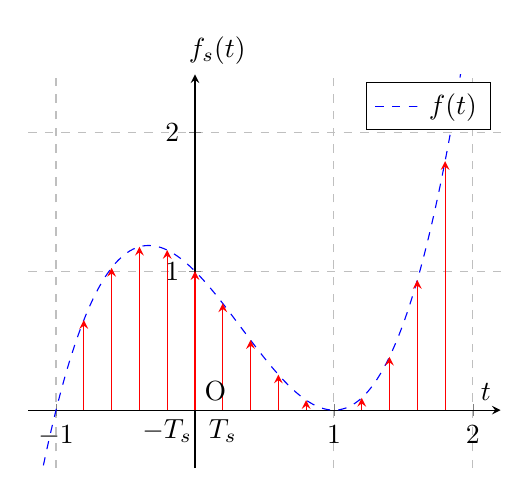
\begin{tikzpicture}
            \begin{axis}[
                axis lines = middle,
                xlabel = {$t$},
                ylabel = {$f_s(t)$},
                ylabel style={at={(rel axis cs:0.4, 1)}, anchor=south},
                xmin = -1.2, xmax = 2.2,
                ymin = -0.2, ymax = 2.2,
                xtick distance = 1,
                ytick distance = 1,
                grid = major,
                grid style = dashed,
                scale only axis,
                width = 6cm,
                height = 5cm,
                axis equal,
            ]
            \addplot[domain=-2.2:2.2, samples=100, smooth, blue, dashed] {(x - 1)^2 * (x + 1)};
            \addlegendentry{$f(t)$}
            \draw[-stealth, red] (axis cs:-0.8, 0) -- (axis cs:-0.8, 0.648);
            \draw[-stealth, red] (axis cs:-0.6, 0) -- (axis cs:-0.6, 1.024);
            \draw[-stealth, red] (axis cs:-0.4, 0) -- (axis cs:-0.4, 1.176);
            \draw[-stealth, red] (axis cs:-0.2, 0) -- (axis cs:-0.2, 1.152);
            \draw[-stealth, red] (axis cs:0, 0) -- (axis cs:0, 1);
            \draw[-stealth, red] (axis cs:0.2, 0) -- (axis cs:0.2, 0.768);
            \draw[-stealth, red] (axis cs:0.4, 0) -- (axis cs:0.4, 0.504);
            \draw[-stealth, red] (axis cs:0.6, 0) -- (axis cs:0.6, 0.256);
            \draw[-stealth, red] (axis cs:0.8, 0) -- (axis cs:0.8, 0.072);
            \draw[-stealth, red] (axis cs:1.2, 0) -- (axis cs:1.2, 0.088);
            \draw[-stealth, red] (axis cs:1.4, 0) -- (axis cs:1.4, 0.384);
            \draw[-stealth, red] (axis cs:1.6, 0) -- (axis cs:1.6, 0.936);
            \draw[-stealth, red] (axis cs:1.8, 0) -- (axis cs:1.8, 1.792);
            \node at (axis cs:0, 0) [anchor=south west] {O};
            \node at (axis cs:-0.2, 0) [anchor=north] {$-T_s$};
            \node at (axis cs:0.2, 0) [anchor=north] {$T_s$};
            \end{axis}
        \end{tikzpicture}
        \caption{抽样信号}
        \label{fig:sampling-signal}
    \end{figure}
\end{example}

\begin{note}
    冲击信号、冲激串和抽样信号之间的关系如图 \ref{fig:impulse-impulse-train-sampled-signal} 所示:
    \begin{figure}[H]
        \centering
        \begin{tikzpicture}
            \node (impulse) [draw, rectangle, minimum width=2cm, minimum height=1cm] at (0, 0) {冲激信号};
            \node (impulse_train) [draw, rectangle, minimum width=2cm, minimum height=1cm] at (5, 0) {冲激串};
            \node (continuous_signal) [draw, rectangle, minimum width=2cm, minimum height=1cm] at (10, 0) {连续信号};
            \node (sampled_signal) [draw, rectangle, minimum width=2cm, minimum height=1cm] at (7.5, -2.5) {抽样信号};
        
            \draw[->, dashed, red] (impulse) -- node[above] {加法} (impulse_train);
            \draw[-] (continuous_signal) -- (impulse_train);
            \draw[->, dashed, red] (7.5, 0) -- node[right, pos=0.5] {乘法} (sampled_signal);
        \end{tikzpicture}
        \caption{冲击信号、冲激串和抽样信号之间的关系}
        \label{fig:impulse-impulse-train-sampled-signal}
    \end{figure}
\end{note}
